%\document{article}
\documentclass[UTF8]{ctexart}
\usepackage{listings} 
\usepackage{amsmath}
\usepackage{graphicx}
\usepackage{fancyhdr}
\usepackage{float}

\title{寄存器文件}
\author{朱河勤   PB16030899}
\pagestyle{fancy}
\lhead{朱河勤   PB16030899}
\chead{寄存器文件}
\rhead{2017/11/23}
\begin{document}
\maketitle
\tableofcontents

\section{实验目的}

\paragraph{1}熟练掌握时序逻辑电路的设计方法

\paragraph{2}掌握寄存器文件的实现原理
\paragraph{3}掌握数码管动态扫描实现方法



\section{设备外设}
时钟(20MHz )、拨动开关(4个, 输入,地址选择)、八段码(4个)

\section{要求}
16*16寄存器文件
\paragraph{*}用模块化设计,实现16*16bit的寄存器文件
\paragraph{*}具备2组读端口及1组写端口
\paragraph{*}通过读端口可从0~15号的任意地址读取数据
\paragraph{*}通过写端口可向0~15号的任意地址写入数据
\paragraph{*}读写端口为全双工的工作方式
\paragraph{*}0~15号寄存器的复位初值依次为:“0x0000,0x1100,0x2200,...,0xFF00”
\paragraph{*}通过1组读端口及写端口,所有寄存器的值每0.5s秒钟加1
\paragraph{*}通过拨动开关做为另1组读端口地址输入,将读出结果以16进制显示在七段数码管上

\section{实验结果}
成功满足要求,能够时分复用降频,能写入读出,并有异步复位功能。\\
仿真结果
\begin{figure}[H]
  \centering
  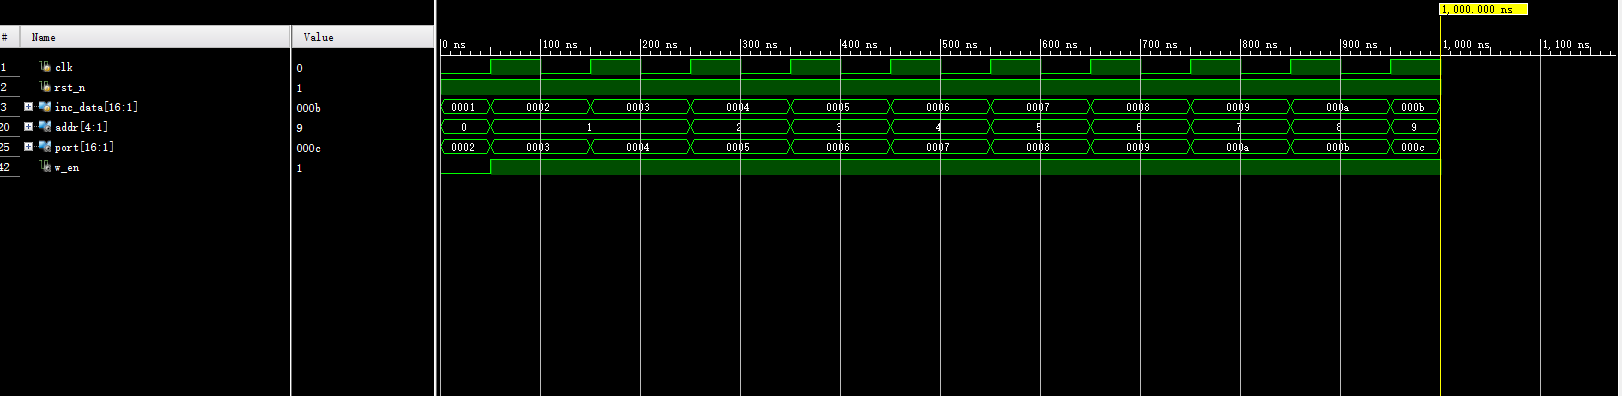
\includegraphics[width=1\textwidth]{inc.png}
\end{figure}


\section{实验分析}
\paragraph{1}由于一次只能亮一个八段码,所以要想到分频时分复用
\paragraph{2}由于每0.5秒一次,所以要有个计数器来计数100000000
\paragraph{3}我犯了一个错误,没计算就直接用20位的reg来储存10000000,结果溢出,导致不能加1,所以要吸取教训
\paragraph{4}实验仿真也不能拘泥,比如仿真时,要检查去毛刺模块,可以把时钟周期数改小

\section{思考题}
对于我的寄存器文件,由于我在写的时候判断是否在读,如果在读,则不写。所以我的寄存器文件在读时不会写。
\section{源代码}

\begin{verbatim}
// top
module top(
        input clk,rst_n, [3:0] addr_r,//bt
        output [2:0] sel,[7:0] tuple
    );
    
    wire [15:0] out;
    wire [1:0] clock;
    wire [15:0]  inc_data;
    wire [15:0] port;
    wire [3:0] addr_w;
    wire w_en;
//    debounce (clk,rst_n,bt,w_en);
    underclocking i1(clk,clock);
    reg_16_16  i2( rst_n ,clk,w_en,addr_r, addr_w, port, out,inc_data);
//    regfile  i5( rst_n ,clk,0,addr_r, addr_w, port, out,inc_data);
    seg i3(clk,rst_n,out,clock,tuple,sel);
    inc i4(clk,rst_n,inc_data,port,addr_w,w_en);
endmodule



//时分复用

module underclocking(
    input clk, 
    output  [2:1] clock_out
    );
    reg [18:1]count2;
    reg [2:1]clock;
    initial begin count2=0; clock=0; end
    assign clock_out = clock;
    always@(negedge clk )
//            if(rst_n);
//                begin
//                count2<=0;
//                end
//            else 
             if(count2==18'd100000)
                begin
                    count2<=18'd0;
                    clock<=clock+2'd1;
                end
            else count2<=count2+18'd1;
endmodule


//寄存器文件

module reg_16_16(
    input rst_n ,clk,w_en,[3:0] addr_r,[3:0] addr_w,[15:0] port,
    output   reg[15:0] port_reg,reg[15:0] inc_data
    );
    reg [15:0] reg0;
    reg [15:0] reg1;
    reg [15:0] reg2;
    reg [15:0] reg3;
    reg [15:0] reg4;
    reg [15:0] reg5;
    reg [15:0] reg6;
    reg [15:0] reg7;
    reg [15:0] reg8;
    reg [15:0] reg9;
    reg [15:0] reg10;
    reg [15:0] reg11;
    reg [15:0] reg12;
    reg [15:0] reg13;
    reg [15:0] reg14;
    reg [15:0] reg15;
    
  
 
   initial begin 
           reg0 = 16'h0000;
           reg1 = 16'h1100;
           reg2 = 16'h2200;
           reg3 = 16'h3300;
           reg4 = 16'h4400;
           reg5 = 16'h5500;
           reg6 = 16'h6600;
           reg7 = 16'h7700;
           reg8 = 16'h8800;
           reg9 = 16'h9900;
           reg10 = 16'hAA00;
           reg11 = 16'hBB00;
           reg12 = 16'hCC00;
           reg13 = 16'hDD00;
           reg14 = 16'hEE00;
           reg15 = 16'hFF00;
       end
    always@(posedge clk,negedge rst_n)
        if(~rst_n )
            begin 
                reg0 = 16'h0000;
                reg1 = 16'h1100;
                reg2 = 16'h2200;
                reg3 = 16'h3300;
                reg4 = 16'h4400;
                reg5 = 16'h5500;
                reg6 = 16'h6600;
                reg7 = 16'h7700;
                reg8 = 16'h8800;
                reg9 = 16'h9900;
                reg10 = 16'hAA00;
                reg11 = 16'hBB00;
                reg12 = 16'hCC00;
                reg13 = 16'hDD00;
                reg14 = 16'hEE00;
                reg15 = 16'hFF00;
            end
     always@(*)
            case(addr_r)
                0: port_reg<= reg0;
                1: port_reg<= reg1;
                2: port_reg<= reg2;
                3: port_reg<= reg3;
                4: port_reg<= reg4;
                5: port_reg<= reg5;
                6: port_reg<= reg6;
                7: port_reg<= reg7;
                8: port_reg<= reg8;
                9: port_reg<= reg9;
                10: port_reg<= reg10;
                11: port_reg<= reg11;
                12: port_reg<= reg12;
                13: port_reg<= reg13;
                14: port_reg<= reg14;
                15: port_reg<= reg15;
            endcase
      always@(*)
            case(addr_w)
                0: inc_data<= reg0;
                1: inc_data<= reg1;
                2: inc_data<= reg2;
                3: inc_data<= reg3;
                4: inc_data<= reg4;
                5: inc_data<= reg5;
                6: inc_data<= reg6;
                7: inc_data<= reg7;
                8: inc_data<= reg8;
                9: inc_data<= reg9;
                10: inc_data<= reg10;
                11: inc_data<= reg11;
                12: inc_data<= reg12;
                13: inc_data<= reg13;
                14: inc_data<= reg14;
                15: inc_data<= reg15;
            endcase    
                        
        
        always@(posedge clk)
            if(w_en)
            case(addr_w)
                0: reg0 <= port;
                1: reg1 <= port;
                2: reg2 <= port;
                3: reg3 <= port;
                4: reg4 <= port;
                5: reg5 <= port;
                6: reg6 <= port;
                7: reg7 <= port;
                8: reg8 <= port;
                9: reg9 <= port;
                10: reg10 <= port;
                11: reg11 <= port;
                12: reg12 <= port;
                13: reg13 <= port;
                14: reg14 <= port;
                15: reg15 <= port;
           endcase

endmodule


//八段码

module seg(
        input clk,rst_n,[15:0] data,[2:1] clock,
        output reg  [7:0] out,reg [2:0] sel
        );
        always@(*)
                case(clock)
                2'b00: begin sel=3'b000;
                        case(data[3:0])    
                             0:out<=8'b1100_0000;
                             1:out<=8'b1111_1001;
                             2:out<=8'b1010_0100;
                             3:out<=8'b1011_0000;                    
                             4:out<=8'b1001_1001;
                             5:out<=8'b1001_0010;
                             6:out<=8'b1000_0010;
                             7:out<=8'b1101_1000;
                             8:out<=8'b1000_0000;
                             9:out<=8'b1001_0000;
                             10:out<=8'b1000_1000;
                             11:out<=8'b1000_0011;
                             12:out<=8'b1100_0110;
                             13:out<=8'b1010_0001;
                             14:out<=8'b1000_0110;
                             15:out<=8'b1000_1110;
                         endcase
                        end
                2'b01: begin sel=3'b001;
                        case(data[7:4])    
                             0:out<=8'b1100_0000;
                             1:out<=8'b1111_1001;
                             2:out<=8'b1010_0100;
                             3:out<=8'b1011_0000;                    
                             4:out<=8'b1001_1001;
                             5:out<=8'b1001_0010;
                             6:out<=8'b1000_0010;
                             7:out<=8'b1101_1000;
                             8:out<=8'b1000_0000;
                             9:out<=8'b1001_0000;
                             10:out<=8'b1000_1000;
                             11:out<=8'b1000_0011;
                             12:out<=8'b1100_0110;
                             13:out<=8'b1010_0001;
                             14:out<=8'b1000_0110;
                             15:out<=8'b1000_1110;
                         endcase
                        end
                2'b10: begin sel=3'b010;
                        case(data[11:8])    
                             0:out<=8'b1100_0000;
                             1:out<=8'b1111_1001;
                             2:out<=8'b1010_0100;
                             3:out<=8'b1011_0000;                    
                             4:out<=8'b1001_1001;
                             5:out<=8'b1001_0010;
                             6:out<=8'b1000_0010;
                             7:out<=8'b1101_1000;
                             8:out<=8'b1000_0000;
                             9:out<=8'b1001_0000;
                             10:out<=8'b1000_1000;
                             11:out<=8'b1000_0011;
                             12:out<=8'b1100_0110;
                             13:out<=8'b1010_0001;
                             14:out<=8'b1000_0110;
                             15:out<=8'b1000_1110;
                         endcase
                        end
                2'b11: begin sel=3'b011;
                        case(data[15:12])    
                             0:out<=8'b1100_0000;
                             1:out<=8'b1111_1001;
                             2:out<=8'b1010_0100;
                             3:out<=8'b1011_0000;                    
                             4:out<=8'b1001_1001;
                             5:out<=8'b1001_0010;
                             6:out<=8'b1000_0010;
                             7:out<=8'b1101_1000;
                             8:out<=8'b1000_0000;
                             9:out<=8'b1001_0000;
                             10:out<=8'b1000_1000;
                             11:out<=8'b1000_0011;
                             12:out<=8'b1100_0110;
                             13:out<=8'b1010_0001;
                             14:out<=8'b1000_0110;
                             15:out<=8'b1000_1110;
                         endcase
                        end
               endcase
                 
endmodule


//计数增加

module inc(
    input clk,rst_n, [15:0] in,
    output reg [15:0] out,
    output reg [3:0] addr,reg w_en
    );    
    reg  [19:0] cnt;
    
    parameter total_times=10_000_000; //clk_20mhz   0.5s    

    initial begin
        cnt = 20'd16;
        w_en=0;
        addr=0;
        
    end
    
    always@(posedge clk,negedge rst_n)
        if(~rst_n||cnt==total_times)cnt=0;
        else begin cnt=cnt+1; addr=cnt[3:0]; end 
     
     always @(posedge clk)
            if(cnt>15)
                w_en<=0;
            else w_en<=1; 
     always @(*) out =in +1;
endmodule
\end{verbatim}


\section{模块划分}
\begin{figure}[H]
  \centering
  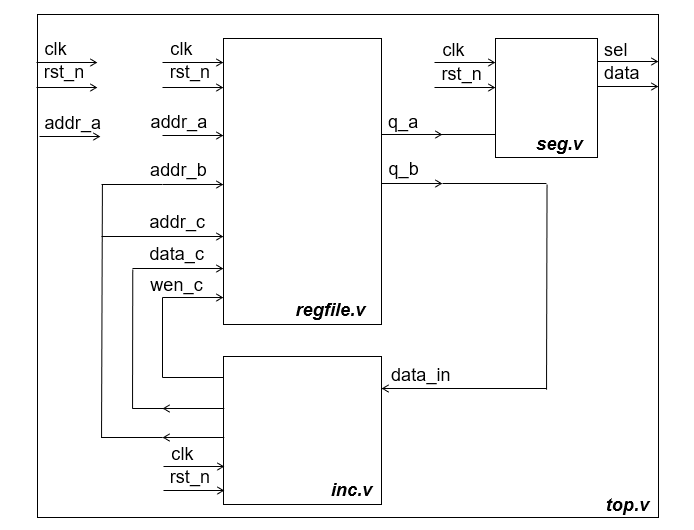
\includegraphics[width=1\textwidth]{module.png}
\end{figure}

\end{document}